\chapter{Stereochemie: chiraliteit en isomeren}\label{ch:g12:stereochemistry}

Blaadjes groene munt en karwijzaad ruiken totaal verschillend: het ene is
de frisse geur van kauwgom, het andere de warme geur van roggebrood. Toch
is het \omterm{def:g7:atoms-and-molecules:molecule}{molecuul} dat voor beide geuren verantwoordelijk is hetzelfde
carvon, opgebouwd uit dezelfde \omterm{def:g7:atoms-and-molecules:atom}{atomen}, in dezelfde volgorde gebonden. De
twee carvonen verschillen alleen zoals een linkerhand verschilt van een
rechterhand: elk is het spiegelbeeld van het andere. Onze neus, die is
opgebouwd uit \omterm{def:g7:atoms-and-molecules:molecule}{moleculen} die zelf ``links- of rechtshandig'' zijn, kan ze
uit elkaar houden. In dit hoofdstuk leer je \omterm{def:g7:atoms-and-molecules:molecule}{moleculen} in drie dimensies
te zien.

\begin{recall}
De vorm van \omterm{def:g7:atoms-and-molecules:molecule}{moleculen}, en de wiggen en streepjes waarmee je ze ruimtelijk
tekent (\cref{ch:g10:lewis-and-shape}). \omterm{def:g11:organic-skeletons:isomer}{Structuurisomeren}
(\cref{ch:g11:organic-skeletons}). \omterm{def:g11:functional-groups:functional-group}{Karakteristieke groepen}
(\cref{ch:g11:functional-groups}).
\end{recall}

\begin{omfigure}
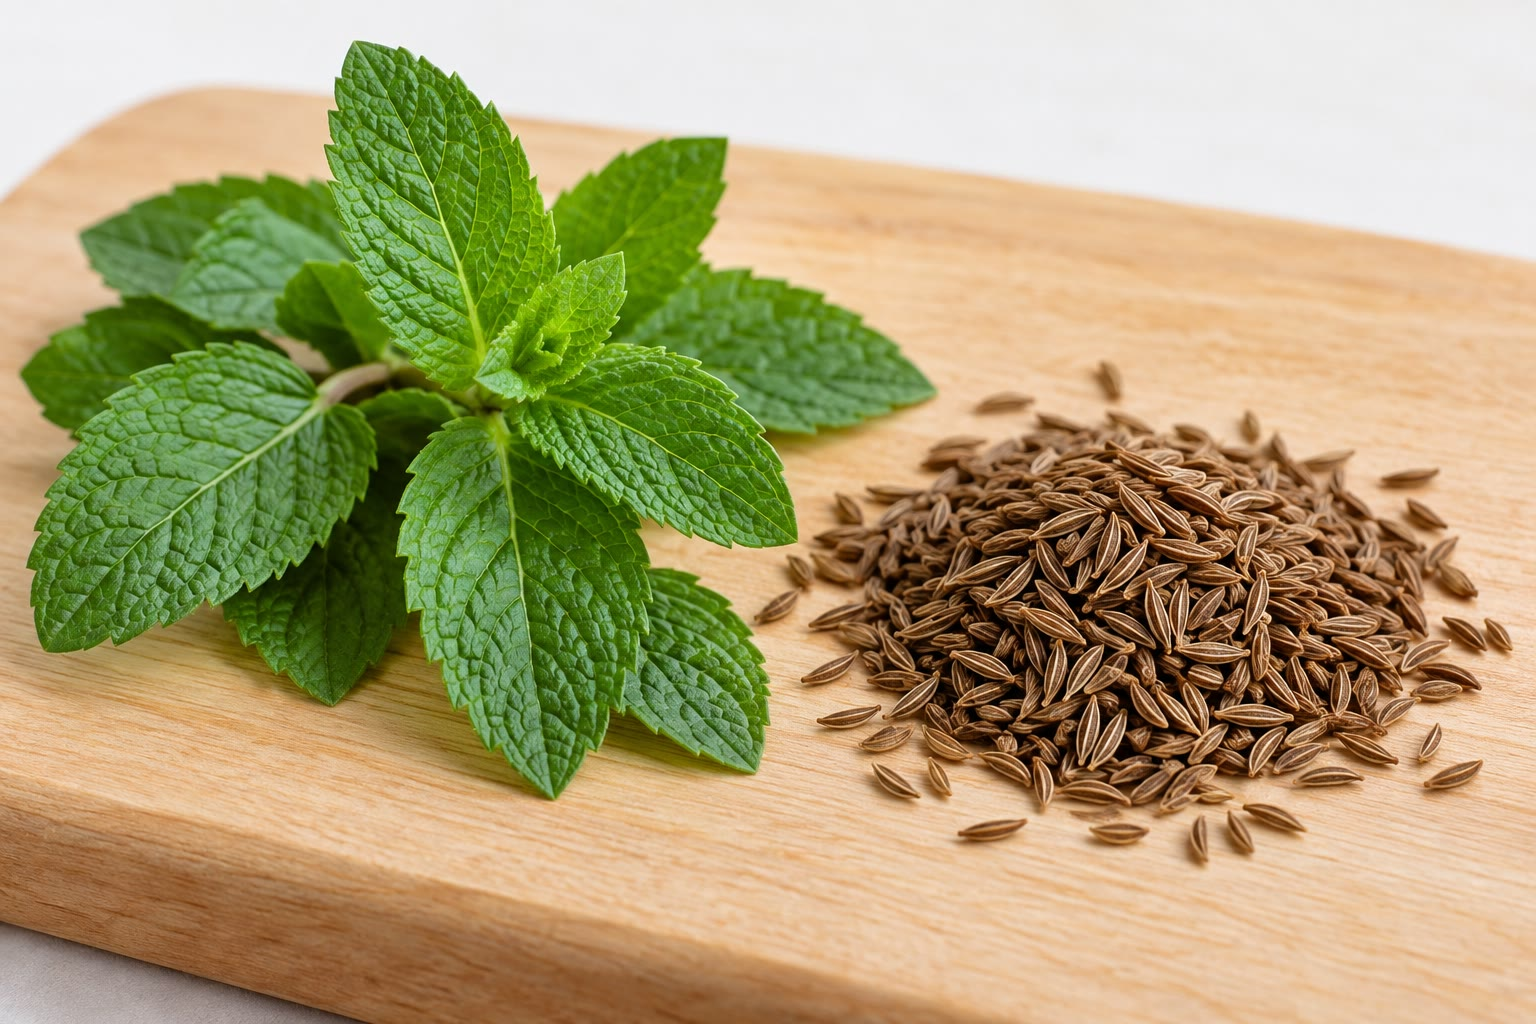
\includegraphics[width=0.48\linewidth]{images/book1/ai/g12-mint-caraway.jpg}

{\small Groene munt en karwij: twee \omterm{def:g7:atoms-and-molecules:molecule}{moleculen} die elkaars spiegelbeeld
zijn, twee geuren.}
\end{omfigure}

\section{Moleculen in de ruimte}

\begin{definition}[Stereo-isomeren]\label{def:g12:stereochemistry:stereoisomer}
\emph{Stereo-isomeren}\index{stereo-isomeren} zijn \omterm{def:g7:atoms-and-molecules:molecule}{moleculen} met dezelfde
formule en dezelfde volgorde van gebonden \omterm{def:g7:atoms-and-molecules:atom}{atomen}, die alleen verschillen
in de ruimtelijke rangschikking van hun \omterm{def:g7:atoms-and-molecules:atom}{atomen}.
\end{definition}

\begin{definition}[Weergave volgens Cram]\label{def:g12:stereochemistry:cram}
In de \emph{weergave volgens Cram}\index{weergave volgens Cram} van een
koolstofatoom met vier enkelvoudige bindingen worden twee bindingen in
het vlak van het papier getekend als gewone lijnen, onder een hoek; de
binding die naar de lezer toe wijst als een volle wig, en de binding die
van de lezer af wijst als een gestreepte wig.
\end{definition}

\section{Chiraliteit}

\begin{definition}[Chiraal, asymmetrisch koolstofatoom]\label{def:g12:stereochemistry:chiral}
Een voorwerp of een \omterm{def:g7:atoms-and-molecules:molecule}{molecuul} is \emph{chiraal}\index{chiraal} als het
niet samen te laten vallen is met zijn spiegelbeeld, zoals een hand. Een
koolstofatoom dat aan vier verschillende \omterm{def:g7:atoms-and-molecules:atom}{atomen} of groepen gebonden is,
is een \emph{asymmetrisch koolstofatoom}\index{asymmetrisch koolstofatoom};
het wordt vaak met een sterretje aangegeven.
\end{definition}

\begin{proposition}[Eén asymmetrisch koolstofatoom maakt een molecuul chiraal]\label{prop:g12:stereochemistry:one-carbon}
Een \omterm{def:g7:atoms-and-molecules:molecule}{molecuul} met precies één \omterm{def:g12:stereochemistry:chiral}{asymmetrisch koolstofatoom} is \omterm{def:g12:stereochemistry:chiral}{chiraal}.
\end{proposition}

\begin{proof}
Aangenomen: twee van de vier verschillende groepen rond het \omterm{def:g12:stereochemistry:chiral}{asymmetrische
koolstofatoom} verwisselen geeft het spiegelbeeld, en geen enkele draaiing
van het hele \omterm{def:g7:atoms-and-molecules:molecule}{molecuul} kan dat terugdraaien, omdat de vier groepen allemaal
verschillend zijn.
\end{proof}

\begin{definition}[Enantiomeren, racemisch mengsel]\label{def:g12:stereochemistry:enantiomer}
Twee \omterm{def:g12:stereochemistry:stereoisomer}{stereo-isomeren} die elkaars spiegelbeeld zijn en niet samen te laten
vallen, zijn \emph{enantiomeren}\index{enantiomeren}. Een \omterm{def:g6:pure-substances-and-mixtures:mixture}{mengsel} van
gelijke hoeveelheden van twee enantiomeren is een \emph{racemisch
mengsel}\index{racemisch mengsel}.
\end{definition}

\begin{omfigure}
\setchemfig{atom sep=2.2em}
\begin{tikzpicture}[font=\small]
  \node at (-2.4,0) {\chemfig{C(-[2]COOH)(-[4]H_3C)(<[:-30]OH)(<:[:-150]H)}};
  \node at (2.4,0) {\chemfig{C(-[2]COOH)(-[0]CH_3)(<[:-150]HO)(<:[:-30]H)}};
  \draw[dashed, omDef, thick] (0,-1.5) -- (0,1.6) node[above] {spiegel};
  \node[anchor=north] at (-2.4,-1.4) {melkzuur, A};
  \node[anchor=north] at (2.4,-1.4) {zijn spiegelbeeld, B};
\end{tikzpicture}

{\small De twee \omterm{def:g12:stereochemistry:enantiomer}{enantiomeren} van melkzuur, \ce{CH3-CH(OH)-COOH}, in de
\omterm{def:g12:stereochemistry:cram}{weergave volgens Cram}. Het centrale koolstofatoom is asymmetrisch
(\ce{H}, \ce{OH}, \ce{CH3}, \ce{COOH}). Geen enkele draaiing maakt van A
B: ze verschillen zoals een linker- en een rechterhand.}
\end{omfigure}

\begin{method}[Is een molecuul chiraal?]\label{met:g12:stereochemistry:chiral}
\begin{enumerate}
  \item Zoek \omterm{def:g12:stereochemistry:chiral}{asymmetrische koolstofatomen}: een koolstofatoom met vier
        verschillende groepen. Geen: het \omterm{def:g7:atoms-and-molecules:molecule}{molecuul} is (in dit boek) niet
        \omterm{def:g12:stereochemistry:chiral}{chiraal}.
  \item Precies één: het \omterm{def:g7:atoms-and-molecules:molecule}{molecuul} is \omterm{def:g12:stereochemistry:chiral}{chiraal}.
  \item Twee of meer: zoek een vlak dat het \omterm{def:g7:atoms-and-molecules:molecule}{molecuul}, in een van zijn
        vormen, in twee spiegelbeeldige helften snijdt; als er zo'n vlak
        is, is het \omterm{def:g7:atoms-and-molecules:molecule}{molecuul} niet \omterm{def:g12:stereochemistry:chiral}{chiraal}, anders wel.
\end{enumerate}
\end{method}

\begin{remark}[Dezelfde eigenschappen, verschillende geuren]\label{rem:g12:stereochemistry:same}
% ledger: smell:carvone-R, smell:carvone-S
Twee \omterm{def:g12:stereochemistry:enantiomer}{enantiomeren} hebben hetzelfde smelt- en kookpunt, dezelfde
\omterm{def:g6:solutions-and-solubility:solubility}{oplosbaarheid} en dezelfde spectra: elke meting met iets wat zelf niet
\omterm{def:g12:stereochemistry:chiral}{chiraal} is, geeft voor beide hetzelfde resultaat. Ze verschillen pas als
ze iets \omterm{def:g12:stereochemistry:chiral}{chiraals} tegenkomen, zoals gepolariseerd licht, dat ze in
tegengestelde richting draaien, of de receptoren van de neus: het ene
carvon ruikt naar groene munt, zijn \omterm{def:g12:stereochemistry:enantiomer}{enantiomeer} naar karwij.
\end{remark}

\section{Diastereomeren}

\begin{definition}[Diastereomeren]\label{def:g12:stereochemistry:diastereomer}
\omterm{def:g12:stereochemistry:stereoisomer}{Stereo-isomeren} die niet elkaars spiegelbeeld zijn, zijn
\emph{diastereomeren}\index{diastereomeren}. Anders dan \omterm{def:g12:stereochemistry:enantiomer}{enantiomeren}
hebben diastereomeren verschillende fysische eigenschappen.
\end{definition}

\begin{proposition}[Stereo-isomeren tellen]\label{prop:g12:stereochemistry:count}
Een \omterm{def:g7:atoms-and-molecules:molecule}{molecuul} met $n$ \omterm{def:g12:stereochemistry:chiral}{asymmetrische koolstofatomen} heeft ten hoogste $2^n$
\omterm{def:g12:stereochemistry:stereoisomer}{stereo-isomeren}. Het zijn er minder als het \omterm{def:g7:atoms-and-molecules:molecule}{molecuul} uit twee gelijke
helften bestaat: dan heeft een van de combinaties een spiegelvlak en is
ze niet \omterm{def:g12:stereochemistry:chiral}{chiraal} (een \emph{meso}-vorm).
\end{proposition}

\begin{proof}
Elk \omterm{def:g12:stereochemistry:chiral}{asymmetrisch koolstofatoom} kan twee rangschikkingen aannemen,
onafhankelijk van de andere: $2 \times 2 \times \dots \times 2 = 2^n$
combinaties. Als twee combinaties hetzelfde \omterm{def:g7:atoms-and-molecules:molecule}{molecuul} zijn, daalt het
aantal.
\end{proof}

\begin{omfigure}
\setchemfig{atom sep=1.9em}
\begin{tabular}{ccc}
\chemfig{HOOC-[:-30]C(<[:-90]OH)-[:30]C(<[:90]OH)-[:-30]COOH} &
\chemfig{HOOC-[:-30]C(<:[:-90]OH)-[:30]C(<:[:90]OH)-[:-30]COOH} &
\chemfig{HOOC-[:-30]C(<[:-90]OH)-[:30]C(<:[:90]OH)-[:-30]COOH} \\[4pt]
\small L-wijnsteenzuur & \small D-wijnsteenzuur & \small meso-wijnsteenzuur \\
\small (\omterm{def:g12:stereochemistry:chiral}{chiraal}) & \small (\omterm{def:g12:stereochemistry:chiral}{chiraal}, spiegelbeeld van L) & \small (niet \omterm{def:g12:stereochemistry:chiral}{chiraal})
\end{tabular}

{\small De drie \omterm{def:g12:stereochemistry:stereoisomer}{stereo-isomeren} van wijnsteenzuur. L en D zijn
\omterm{def:g12:stereochemistry:enantiomer}{enantiomeren}; elk is een \omterm{def:g12:stereochemistry:diastereomer}{diastereomeer} van de meso-vorm, die in een van
haar vormen een spiegelvlak heeft: drie \omterm{def:g12:stereochemistry:stereoisomer}{stereo-isomeren}, niet
$2^2 = 4$.}
\end{omfigure}

\begin{history}[Pasteur sorteert kristallen met de hand, 1848]
In 1848 bekeek de jonge scheikundige Louis Pasteur met een vergrootglas
kristallen van een zout van ``druivenzuur'', een vorm van wijnsteenzuur
die gepolariseerd licht geen kant op draaide. Hij zag dat de kristallen
in twee vormen voorkwamen, elkaars spiegelbeeld, en sorteerde ze een
voor een met een pincet. Opgelost draaide het ene hoopje gepolariseerd
licht naar rechts en het andere, over dezelfde hoek, naar links:
druivenzuur was een \omterm{def:g6:pure-substances-and-mixtures:mixture}{mengsel} van twee \omterm{def:g7:atoms-and-molecules:molecule}{moleculen} die elkaars spiegelbeeld
zijn. \omterm{def:g7:atoms-and-molecules:molecule}{Moleculen}, concludeerde hij, kunnen links- of rechtshandig zijn.
\end{history}

\begin{omfigure}
\begin{minipage}[t]{0.36\linewidth}\centering
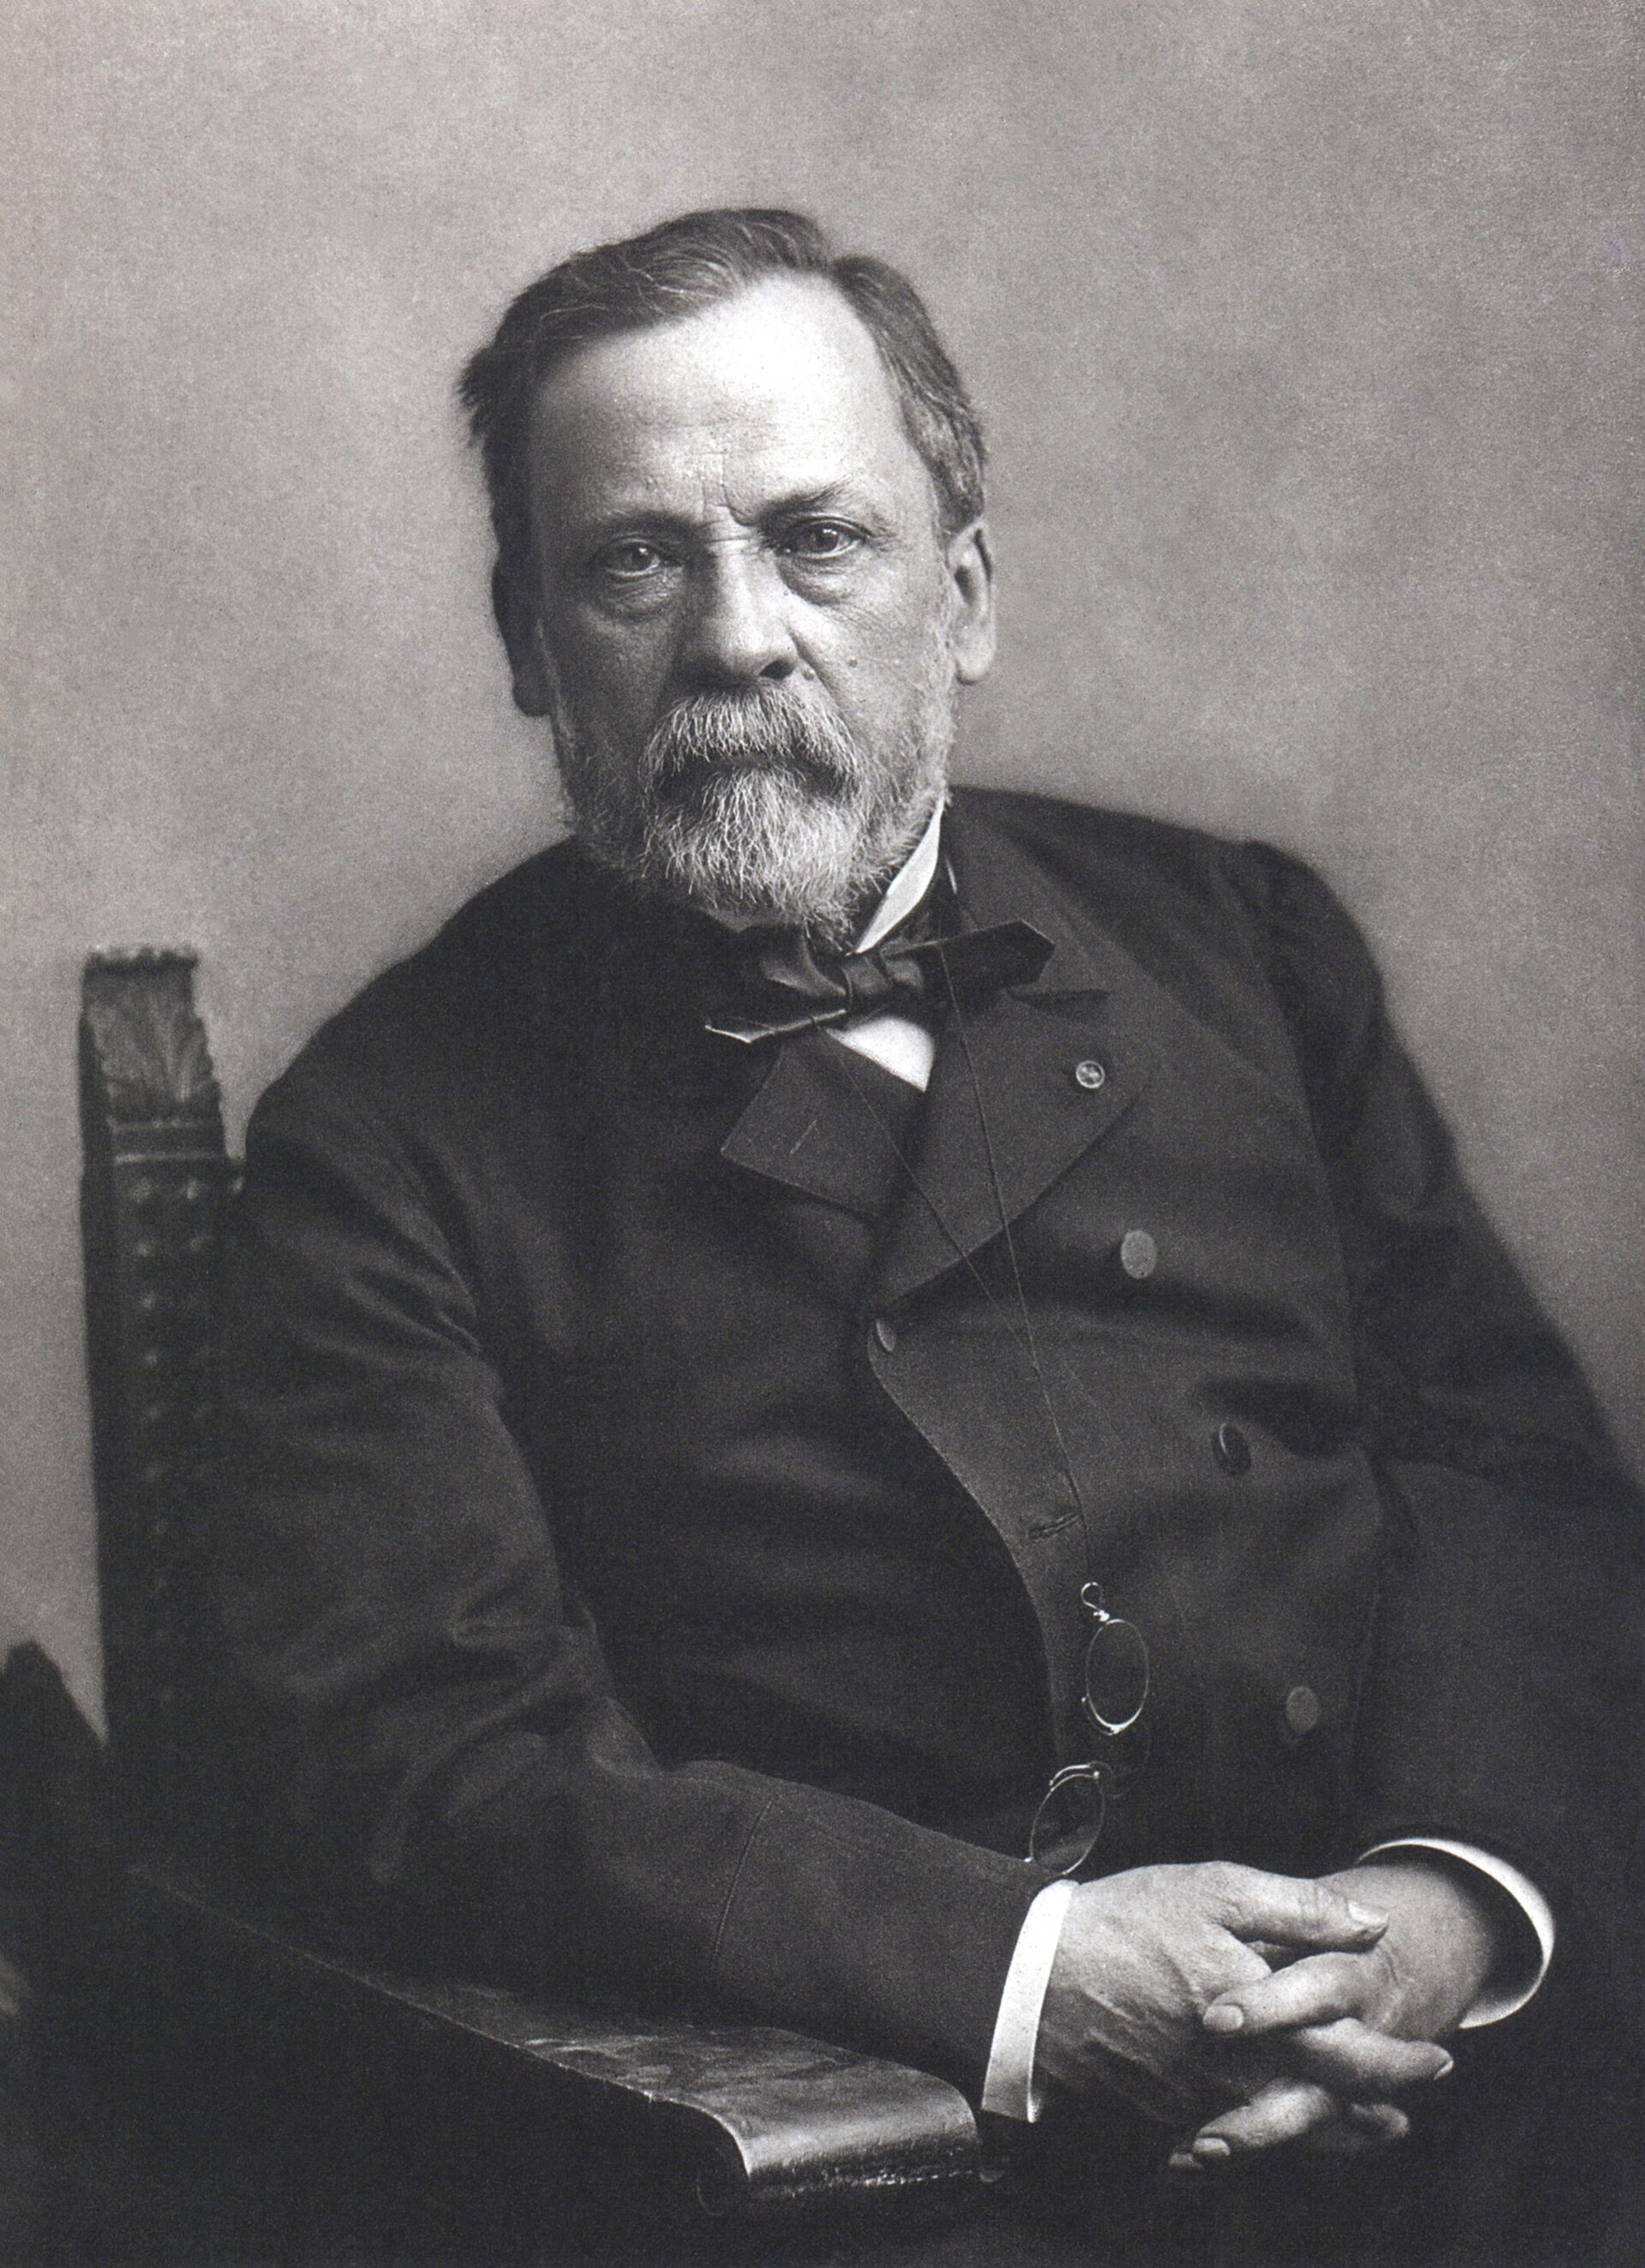
\includegraphics[height=5cm]{images/book1/pasteur.jpg}

{\small Louis Pasteur (1822--1895), gefotografeerd door Paul Nadar.}
\end{minipage}\qquad
\begin{minipage}[t]{0.36\linewidth}\centering
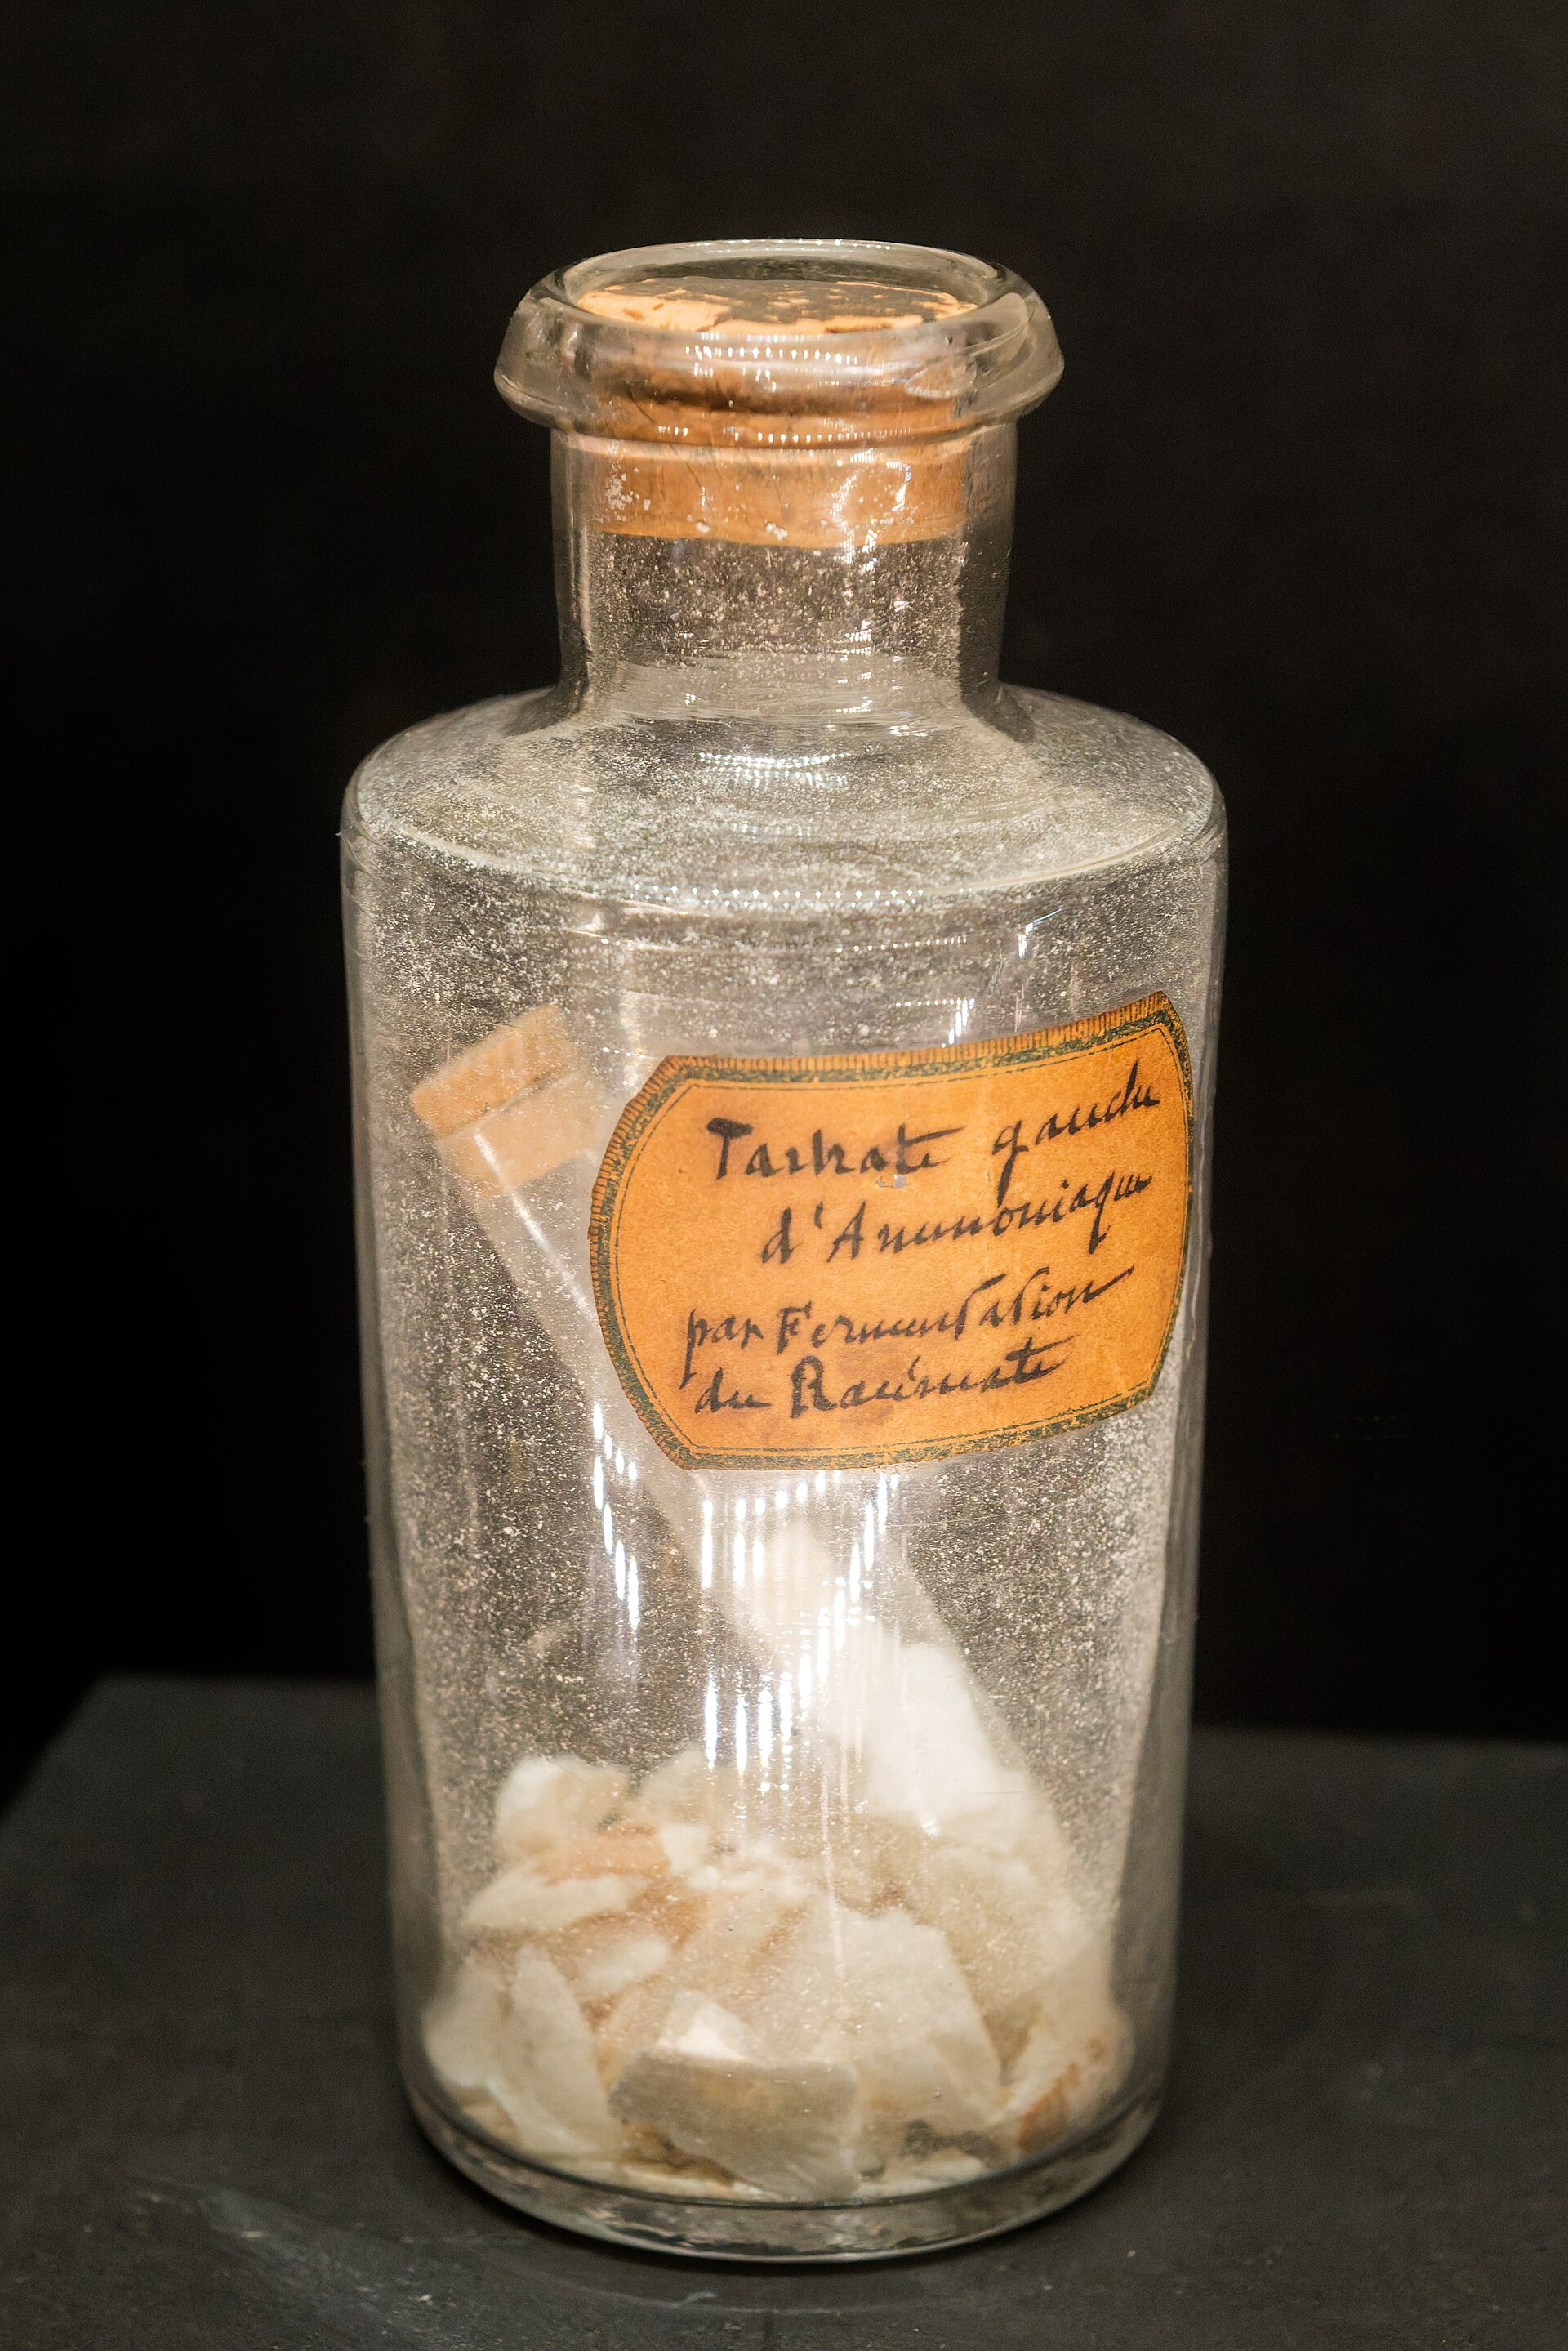
\includegraphics[height=5cm]{images/book1/tartrate-crystals.jpg}

{\small Kristallen van ammoniumtartraat uit de collectie van Pasteur.
Foto Marie-Lan Taÿ Pamart, CC BY 4.0.}
\end{minipage}
\end{omfigure}

\section{Z- en E-isomeren}


\begin{definition}[Z- en E-isomeren]\label{def:g12:stereochemistry:z-e}
Als elk koolstofatoom van een \omterm{def:g10:lewis-and-shape:multiple-bond}{dubbele binding} \ce{C=C} twee verschillende
\omterm{def:g7:atoms-and-molecules:atom}{atomen} of groepen draagt, bestaan er twee \omterm{def:g12:stereochemistry:stereoisomer}{stereo-isomeren}, omdat de
\omterm{def:g10:lewis-and-shape:multiple-bond}{dubbele binding} niet kan draaien. Op elk koolstofatoom heeft de groep
waarvan het gebonden \omterm{def:g7:atoms-and-molecules:atom}{atoom} het grootste \omterm{def:g9:inside-the-atom:atomic-number}{atoomnummer} heeft, voorrang. Als
de twee voorrangsgroepen aan dezelfde kant van de \omterm{def:g10:lewis-and-shape:multiple-bond}{dubbele binding} zitten,
is het \omterm{def:g11:organic-skeletons:isomer}{isomeer} \emph{Z}\index{Z-isomeer}; zitten ze aan tegenovergestelde
kanten, dan is het \emph{E}\index{E-isomeer}.
\end{definition}

\begin{method}[Z of E?]\label{met:g12:stereochemistry:z-e}
\begin{enumerate}
  \item Controleer dat elk koolstofatoom van de \omterm{def:g10:lewis-and-shape:multiple-bond}{dubbele binding} twee
        verschillende groepen draagt; anders is er geen \omterm{def:g12:stereochemistry:z-e}{Z}/E-isomerie.
  \item Geef op elk koolstofatoom voorrang aan de groep waarvan het eerste
        \omterm{def:g7:atoms-and-molecules:atom}{atoom} het grootste \omterm{def:g9:inside-the-atom:atomic-number}{atoomnummer} heeft (de volledige regels voor
        gelijke gevallen staan in het deel voor het eerste
        universiteitsjaar).
  \item Dezelfde kant: \omterm{def:g12:stereochemistry:z-e}{Z}. Tegenovergestelde kanten: \omterm{def:g12:stereochemistry:z-e}{E}.
\end{enumerate}
\end{method}

\begin{omfigure}
\setchemfig{atom sep=2em}
\begin{tabular}{cc}
\chemfig{C(-[:150]H_3C)(-[:210]H)=C(-[:30]CH_3)(-[:-30]H)} &
\chemfig{C(-[:150]H_3C)(-[:210]H)=C(-[:30]H)(-[:-30]CH_3)} \\[4pt]
\small (\omterm{def:g12:stereochemistry:z-e}{Z})-but-2-een: \ce{CH3}-groepen aan dezelfde kant &
\small (\omterm{def:g12:stereochemistry:z-e}{E})-but-2-een: \ce{CH3}-groepen tegenover elkaar
\end{tabular}

{\small De twee \omterm{def:g12:stereochemistry:stereoisomer}{stereo-isomeren} van but-2-een. Op elk koolstofatoom heeft
\ce{CH3} (koolstof, $Z = 6$) voorrang op \ce{H} ($Z = 1$). Het zijn
\omterm{def:g12:stereochemistry:diastereomer}{diastereomeren}: ze koken bij verschillende temperaturen.}
\end{omfigure}

\section{Conformaties}

\begin{definition}[Conformatie]\label{def:g12:stereochemistry:conformation}
De \omterm{def:g7:atoms-and-molecules:atom}{atomen} van een \omterm{def:g7:atoms-and-molecules:molecule}{molecuul} kunnen draaien om een enkelvoudige binding.
Elke rangschikking die je door zulke draaiingen bereikt, is een
\emph{conformatie}\index{conformatie} van het \omterm{def:g7:atoms-and-molecules:molecule}{molecuul}. Conformaties van
één \omterm{def:g7:atoms-and-molecules:molecule}{molecuul} zijn geen \omterm{def:g11:organic-skeletons:isomer}{isomeren}: bij kamertemperatuur gaan ze voortdurend
in elkaar over.
\end{definition}

\begin{omfigure}
\begin{tikzpicture}[font=\small]
  \pic (s) at (0,0) {omnewman={90}{30}};
  \foreach \k in {1,2,3} { \node at (s-f\k) {H}; \node at (s-b\k) {H}; }
  \node[anchor=north, align=center] at (0,-1.7) {gestaffeld: de H-atomen\\ van beide koolstofatomen\\ wisselen elkaar af};
  \pic (e) at (5,0) {omnewman={90}{112}};
  \foreach \k in {1,2,3} { \node at (e-f\k) {H}; \node[black!60] at (e-b\k) {H}; }
  \node[anchor=north, align=center] at (5,-1.7) {eclips: ze staan\\ tegenover elkaar (iets\\ uit elkaar getekend)};
\end{tikzpicture}

{\small Twee \omterm{def:g12:stereochemistry:conformation}{conformaties} van ethaan, \ce{CH3-CH3}, gezien langs de
\ce{C-C}-binding: het voorste koolstofatoom is het middelpunt, het
achterste de cirkel. De gestaffelde \omterm{def:g12:stereochemistry:conformation}{conformatie}, waarin de \omterm{def:g7:atoms-and-molecules:atom}{atomen} het
verst van elkaar af zitten, is het stabielst.}
\end{omfigure}

\begin{remark}[Waarom het ertoe doet]\label{rem:g12:stereochemistry:matters}
Levende wezens zijn opgebouwd uit \omterm{def:g12:stereochemistry:chiral}{chirale} \omterm{def:g7:atoms-and-molecules:molecule}{moleculen} (eiwitten, suikers),
en de receptoren en enzymen die daaruit bestaan, onderscheiden
\omterm{def:g12:stereochemistry:enantiomer}{enantiomeren}: twee \omterm{def:g12:stereochemistry:enantiomer}{enantiomeren} kunnen heel verschillend ruiken, smaken
of als geneesmiddel werken. Daarom moeten scheikundigen die een
geneesmiddel met een \omterm{def:g12:stereochemistry:chiral}{asymmetrisch koolstofatoom} maken, weten welk
\omterm{def:g12:stereochemistry:enantiomer}{enantiomeer} ze maken, en elk afzonderlijk testen.
\end{remark}

\section{Oefeningen}

\begin{exercise}[$\star$]\label{exo:g12:stereochemistry:1}
Welke van deze \omterm{def:g7:atoms-and-molecules:molecule}{moleculen} hebben een \omterm{def:g12:stereochemistry:chiral}{asymmetrisch koolstofatoom}? Geef het
aan met een sterretje. Butaan-2-ol \ce{CH3-CH(OH)-CH2-CH3}; propaan-2-ol
\ce{CH3-CH(OH)-CH3}; 2-chloorbutaan; melkzuur \ce{CH3-CH(OH)-COOH}.
\end{exercise}

\begin{exercise}[$\star$]\label{exo:g12:stereochemistry:2}
Is elk \omterm{def:g11:organic-skeletons:isomer}{isomeer} \omterm{def:g12:stereochemistry:z-e}{Z} of \omterm{def:g12:stereochemistry:z-e}{E}?
\begin{center}
\setchemfig{atom sep=1.8em}
\chemfig{C(-[:150]Cl)(-[:210]H)=C(-[:30]Cl)(-[:-30]H)} \qquad
\chemfig{C(-[:150]H_3C)(-[:210]H)=C(-[:30]H)(-[:-30]CH_2-CH_3)}
\end{center}
\end{exercise}

\begin{exercise}[$\star$]\label{exo:g12:stereochemistry:3}
Welke zijn \omterm{def:g12:stereochemistry:chiral}{chiraal}: een handschoen, een lepel, een schroef, een kubus?
Welk van de \omterm{def:g7:atoms-and-molecules:molecule}{moleculen} \ce{CH2Cl2} en \ce{CHFClBr} is \omterm{def:g12:stereochemistry:chiral}{chiraal}?
\end{exercise}

\begin{exercise}[$\star$]\label{exo:g12:stereochemistry:4}
Wat is een \omterm{def:g12:stereochemistry:enantiomer}{racemisch mengsel}? Ruikt het, in het geval van carvon, naar
groene munt, naar karwij, of naar allebei?
\end{exercise}

\begin{exercise}[$\star$]\label{exo:g12:stereochemistry:5}
Kan but-1-een \ce{CH2=CH-CH2-CH3} als Z- en \omterm{def:g12:stereochemistry:z-e}{E-isomeer} bestaan? Waarom?
\end{exercise}

\begin{exercise}[$\star\star$]\label{exo:g12:stereochemistry:6}
Teken de twee \omterm{def:g12:stereochemistry:enantiomer}{enantiomeren} van butaan-2-ol in de \omterm{def:g12:stereochemistry:cram}{weergave volgens Cram},
met een spiegel ertussen.
\end{exercise}

\begin{exercise}[$\star\star$]\label{exo:g12:stereochemistry:7}
Hoeveel \omterm{def:g12:stereochemistry:stereoisomer}{stereo-isomeren} hebben: 2-chloorbutaan;
2,3-dichloorbutaan \ce{CH3-CHCl-CHCl-CH3}; pent-2-een
\ce{CH3-CH=CH-CH2-CH3}?
\end{exercise}

\begin{exercise}[$\star\star$]\label{exo:g12:stereochemistry:8}
Zeg of deze paren \omterm{def:g12:stereochemistry:enantiomer}{enantiomeren}, \omterm{def:g12:stereochemistry:diastereomer}{diastereomeren} of hetzelfde \omterm{def:g7:atoms-and-molecules:molecule}{molecuul}
zijn: L- en D-wijnsteenzuur; L- en meso-wijnsteenzuur; (\omterm{def:g12:stereochemistry:z-e}{Z})- en
(\omterm{def:g12:stereochemistry:z-e}{E})-but-2-een; meso-wijnsteenzuur en zijn eigen spiegelbeeld.
\end{exercise}

\begin{exercise}[$\star\star$]\label{exo:g12:stereochemistry:9}
Butaan, \ce{CH3-CH2-CH2-CH3}, gezien langs zijn middelste binding. Teken
de gestaffelde \omterm{def:g12:stereochemistry:conformation}{conformatie} waarin de twee \ce{CH3}-groepen tegenover
elkaar staan, en een eclipsconformatie waarin ze naar elkaar toe wijzen.
Welke is het stabielst? Waarom?
\end{exercise}

\begin{exercise}[$\star\star$]\label{exo:g12:stereochemistry:10}
Meso-wijnsteenzuur heeft twee \omterm{def:g12:stereochemistry:chiral}{asymmetrische koolstofatomen}, maar is niet
\omterm{def:g12:stereochemistry:chiral}{chiraal}. Leg dat uit met zijn spiegelvlak.
\end{exercise}

\begin{exercise}[$\star\star$]\label{exo:g12:stereochemistry:11}
Teken en benoem het Z- en het \omterm{def:g12:stereochemistry:z-e}{E-isomeer} van pent-2-een.
\end{exercise}

\begin{exercise}[$\star\star\star$]\label{exo:g12:stereochemistry:12}
2,3-Dibroombutaan \ce{CH3-CHBr-CHBr-CH3} heeft twee \omterm{def:g12:stereochemistry:chiral}{asymmetrische
koolstofatomen}. Teken zijn \omterm{def:g12:stereochemistry:stereoisomer}{stereo-isomeren} in de zigzagweergave die voor
wijnsteenzuur gebruikt is, en laat zien dat een ervan een meso-vorm is.
\end{exercise}

\begin{exercise}[$\star\star\star$]\label{exo:g12:stereochemistry:13}
Een geneesmiddelmolecuul heeft één \omterm{def:g12:stereochemistry:chiral}{asymmetrisch koolstofatoom}. De
\omterm{def:g10:synthesis-yield:synthesis}{synthese} levert een \omterm{def:g12:stereochemistry:enantiomer}{racemisch mengsel}, maar alleen één \omterm{def:g12:stereochemistry:enantiomer}{enantiomeer} past
op de \omterm{def:g12:stereochemistry:chiral}{chirale} receptor waarop het moet werken. Welk deel van het
racemische geneesmiddel is werkzaam? Geef twee manieren waarop een
scheikundige het beter kan doen.
\end{exercise}

\begin{exercise}[$\star\star\star$]\label{exo:g12:stereochemistry:14}
Hexa-2,4-dieen, \ce{CH3-CH=CH-CH=CH-CH3}, heeft twee \omterm{def:g10:lewis-and-shape:multiple-bond}{dubbele bindingen},
die elk \omterm{def:g12:stereochemistry:z-e}{Z} of \omterm{def:g12:stereochemistry:z-e}{E} kunnen zijn. Hoeveel \omterm{def:g12:stereochemistry:stereoisomer}{stereo-isomeren} heeft het? (Let op
de symmetrie van het \omterm{def:g7:atoms-and-molecules:molecule}{molecuul}.)
\end{exercise}

\begin{exercise}[$\star\star\star$]\label{exo:g12:stereochemistry:15}
Een suikermolecuul heeft drie \omterm{def:g12:stereochemistry:chiral}{asymmetrische koolstofatomen} en geen
symmetrie. Hoeveel \omterm{def:g12:stereochemistry:stereoisomer}{stereo-isomeren} kan het ten hoogste hebben? Hoeveel
paren \omterm{def:g12:stereochemistry:enantiomer}{enantiomeren} zijn dat? Hoeveel \omterm{def:g12:stereochemistry:diastereomer}{diastereomeren} heeft elk
\omterm{def:g12:stereochemistry:stereoisomer}{stereo-isomeer}?
\end{exercise}

\section{Probleem: De kristallen van Pasteur}


\begin{problem}[{Weekendprobleem --- wijnsteenzuur heeft twee
asymmetrische koolstofatomen: hoeveel stereo-isomeren heeft het echt?}]
\label{pb:g12:stereochemistry:1}
% ledger: mp:tartaric-L, aw:C, aw:H, aw:O
De vormen van wijnsteenzuur, \ce{HOOC-CH(OH)-CH(OH)-COOH}, speelden een
beslissende rol in de ontdekking dat \omterm{def:g7:atoms-and-molecules:molecule}{moleculen} links- of rechtshandig
kunnen zijn. L-Wijnsteenzuur smelt bij ongeveer \qty{169}{\celsius}.

\medskip
\noindent\textbf{Deel I --- Het \omterm{def:g7:atoms-and-molecules:molecule}{molecuul}.}
\begin{enumerate}
  \item Geef de \omterm{def:g11:organic-skeletons:formulas}{molecuulformule} van wijnsteenzuur en zijn \omterm{def:g10:the-mole:molar-mass}{molaire massa}.
  \item Noem zijn \omterm{def:g11:functional-groups:functional-group}{karakteristieke groepen}, en zeg hoeveel van elk.
  \item Welke koolstofatomen zijn asymmetrisch? Noem van elk de vier
        groepen.
  \item Hoeveel \omterm{def:g12:stereochemistry:stereoisomer}{stereo-isomeren} zou het volgens de regel van dit
        hoofdstuk ten hoogste kunnen hebben?
\end{enumerate}

\medskip
\noindent\textbf{Deel II --- De \omterm{def:g12:stereochemistry:stereoisomer}{stereo-isomeren}.}
\begin{enumerate}[resume]
  \item Zijn in de zigzagtekening van L-wijnsteenzuur de \ce{OH}-groepen
        met volle of met gestreepte wiggen getekend?
  \item Teken zijn spiegelbeeld. Kunnen de twee samenvallen? Geef de naam
        van het spiegelbeeld.
  \item Teken de vorm met één volle en één gestreepte wig. Draai hem in
        gedachten om de middelste binding, en zoek een spiegelvlak.
  \item Is deze vorm \omterm{def:g12:stereochemistry:chiral}{chiraal}? Hoe heet hij?
  \item Leg uit waarom wijnsteenzuur maar drie \omterm{def:g12:stereochemistry:stereoisomer}{stereo-isomeren} heeft.
  \item Zeg of L en D, en daarna L en meso, \omterm{def:g12:stereochemistry:enantiomer}{enantiomeren} of
        \omterm{def:g12:stereochemistry:diastereomer}{diastereomeren} zijn.
\end{enumerate}

\medskip
\noindent\textbf{Deel III --- Eigenschappen.}
\begin{enumerate}[resume]
  \item Bij welke temperatuur smelt D-wijnsteenzuur? Waarom?
  \item Moet meso-wijnsteenzuur bij dezelfde temperatuur smelten? Waarom?
  \item Carvon laat zien dat twee \omterm{def:g12:stereochemistry:enantiomer}{enantiomeren} verschillend kunnen ruiken.
        Waarom kan een neus ze uit elkaar houden en een thermometer niet?
  \item Een \omterm{def:g12:stereochemistry:enantiomer}{racemisch mengsel} van L- en D-wijnsteenzuur: is dat een
        \omterm{def:g6:pure-substances-and-mixtures:pure-substance}{zuivere stof}? Is het als geheel optisch actief?
\end{enumerate}

\medskip
\noindent\textbf{Deel IV --- Pasteur.}
\begin{enumerate}[resume]
  \item Het racemische zout van Pasteur gaf kristallen in twee vormen die
        elkaars spiegelbeeld zijn. Wat bevatte elk kristal?
  \item Welke massa van elke soort kristal kon hij verwachten uit
        \qty{10.0}{g} racemisch zout?
  \item Waarom komt de meso-vorm nooit voor tussen deze kristallen?
  \item Hoe kon hij na het sorteren controleren dat de twee hoopjes
        \omterm{def:g12:stereochemistry:enantiomer}{enantiomeren} waren?
  \item 3-Chloorbutaan-2-ol, \ce{CH3-CHCl-CH(OH)-CH3}, heeft ook twee
        \omterm{def:g12:stereochemistry:chiral}{asymmetrische koolstofatomen}. Hoeveel \omterm{def:g12:stereochemistry:stereoisomer}{stereo-isomeren} heeft het?
        Waarom verliest het er niet een, zoals wijnsteenzuur?
  \item Geef het eindantwoord: hoeveel \omterm{def:g12:stereochemistry:stereoisomer}{stereo-isomeren} heeft
        wijnsteenzuur?
\end{enumerate}
\end{problem}
